\problemname{Dans}
Þegar Forritunarkeppni Framhaldskólanna var haldin á 19.\ öld voru hefðirnar
aðrar en í dag. Til að mynda var tekið fyrir allt sælgæti og það sem teldist
til óhollustu. Keppnin var haldin samhliða Þorrablóti og átu keppendur þorramat
á meðan keppninni stóð og var hver hákarlsbiti talinn sem stig fyrir liðin í
keppninni. Því voru nokkur lið í gegnum árin (1867, 1897, 1899) sem sigruðu keppnina fyrir það
eitt að hafa borðað óhóflegt magn af hákarli.

Ein sú hefð sem glataðist í gegnum aldanna rás var dansleikur Forritunarkeppni
Framhaldskólanna. Sá dansleikur var einn sá virtasti á landinu árum áður og var
stjórnaður af Hallgrími nokkrum. Hallgrímur hafði gaman af einföldum dansformum
og þá sérstaklega vikivaka. Vikivaki er hringdans þar sem þátttakendur haldast í hendur og taka
ákveðin spor í takt við tónlistina en Hallgrími finnst gaman að hafa nokkrar
flækjur í dansinum. Eftir hvert viðlag í laginu sem dansað er við, hefur
Hallgrímur ákveðið að láta suma þátttakendur færa sig um í hringnum.

Þessar breytingar Hallgríms á staðsetningum þátttakendanna lýsa sér þannig að
Hallgrímur gefur fyrir hverja staðsetningu $i$ í hringnum, staðsetninguna á
þeirri manneskju sem á að vera þar eftir næsta viðlag.  Sem dæmi, segjum að
Hallgrímur ákveði að manneskjan í staðsetningu $3$ eigi að fara í staðsetningu
$1$ í hringnum, manneskjan í $1$ eigi að fara í $2$ og manneskjan í $2$ eigi að
fara í $3$, þá lýsir hann þessu á forminu $3~1~2$.

Hallgrímur hefur ákveðið að halda dansleikinn aftur í ár og vill vita fyrir
einhverja ákveðna staðsetningavörpun, hvar hver þátttakandi verður staðsettur í
hringnum eftir nákvæmlega $k$ viðlög.  Eins og vanalega, þá er einfaldast að
kalla í einhvern tölvusnilling til að skrifa forrit sem leysir þetta og hefur
þú verið kallaður til verksins!

\section*{Inntak}
Inntakið inniheldur nákvæmlega tvær línur.  Sú fyrri inniheldur tvær heiltölur
$N$ og $K$ og sú seinni samanstendur af $N$ heiltölum $\pi_1 \pi_2 \dotsc \pi_N$.
Þar táknar tala númer $i$, $\pi_i$, að manneskjan í staðsetningu $\pi_i$ eigi að
vera í staðsetningu $i$ í hringnum eftir næsta viðlag.
Þessi seinni lína inniheldur
eingöngu tölur frá $1$ upp í $N$ og hver tala kemur bara fyrir einu sinni.

\section*{Úttak}
Prentið út á einni línu $N$ tölur, $\rho_1 \rho_2 \dotsc \rho_N$ aðskildar með
einu bili, sem tákna að manneskjan sem byrjaði í staðsetningu $\rho_i$
endaði í staðsetningu $i$ eftir eftir $K$ viðlög.

\section*{Útskýring á sýnidæmum}
Í fyrsta sýnidæminu eru þrjár manneskjur í hringnum og eru tvö viðlög dönsuð.
Eftir fyrsta viðlagið er manneskjan í sæti $3$ komin í $1$, manneskjan í $2$
komin í $1$ og $1$ í $3$. Eftir seinna viðlagið fer manneskjan sem nú er í sæti
$2$ (upphaflega í $3$) í $1$, manneskjan í $3$ (upphaflega $1$) fer í $2$ og
manneskjan sem nú er í $1$ (upphaflega $2$) fer í $3$. Því er lokaúttakið $3~1~2$.

\begin{figure}[!h]
  \centering
  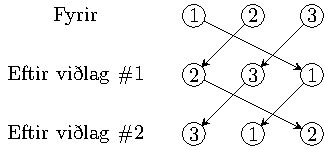
\includegraphics[width=0.6\textwidth] {figures/fig1.pdf}
\end{figure}

Samskonar mynd og fyrir fyrsta sýnidæmið má síðan sjá hér að neðan fyrir þriðja sýnidæmið.
\begin{figure}[!h]
  \centering
  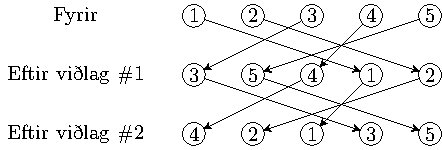
\includegraphics[width=0.6\textwidth] {figures/fig2.pdf}
\end{figure}

\section*{Stigagjöf}

\begin{tabular}{|l|l|l|}
\hline
Hópur & Stig & Inntaksstærð \\ \hline
1 & 10 & $1 \leq N \leq 2,\,0 \leq K \leq 10$ \\ \hline
2 & 40 & $1 \leq N \leq 10,\,0 \leq K \leq 10$ \\ \hline
3 & 25 & $1 \leq N \leq 2,\,0 \leq K \leq 10^9$ \\ \hline
4 & 25 & $1 \leq N \leq 1\,000,\,0 \leq K \leq 10^9$ \\ \hline
\end{tabular}
